% -*- coding: utf-8 -*-
% 2026 Lecture 2. Adapted from lecture-2-3.tex (2025).
% Build from lecture/: xelatex -halt-on-error lecture-2-2-2026.tex
% Keep the 2025 masters and their shared fragments unchanged.
\documentclass[10pt,aspectratio=169]{beamer}
\usepackage[no-math]{fontspec}
\usepackage{amsmath}
\setsansfont{BIZ UDPGothic}
\setmainfont{BIZ UDPGothic}
\XeTeXlinebreaklocale "ja"
\XeTeXlinebreakskip=0pt plus 1pt
\usetheme{Antibes}
\usecolortheme{rose}
\usefonttheme[onlymath]{serif}
\usepackage{unicode-math}
\setmathfont{Latin Modern Math}
\setbeamertemplate{navigation symbols}{}
\setbeamertemplate{footline}[frame number]
\title{計算機実験II (L2)}
\subtitle{分子動力学と統計的サンプリング}
\author{藤堂眞治}
\date{2026/10/23}

\begin{document}
\begin{frame}
  \titlepage
\end{frame}

\begin{frame}{本日の到達目標}
\begin{itemize}
\item 運動方程式の時間積分と、平衡分布からのサンプリングを区別する
\item 速度ベルレ法を実装し、刻み幅と保存量を使って検証する
\item 温度の平均値だけでなく、分布とゆらぎを確認する
\item 力学による提案とMetropolis採択を組み合わせ、HMCを構成する
\end{itemize}
\end{frame}

\begin{frame}{講義1・実習1とのつながり}
\begin{itemize}
\item 前回：カノニカル分布、詳細つりあい、Metropolis法
\item 小さな提案では自己相関が残り、大きな提案では棄却が増える
\item 今回：勾配（力）を利用して、遠くまで移動する提案をつくる
\item 平衡化・自己相関・ビニングによる誤差評価は引き続き必要
\end{itemize}
\[
\pi(q)\propto e^{-\beta U(q)},\qquad
\beta=\frac{1}{k_{\mathrm B}T}
\]
\end{frame}

\section{分子動力学とアンサンブル}

% Adapted from molecular_dynamics-15.tex.
\begin{frame}{古典多粒子系}
\[
H(q,p)=K(p)+U(q),\qquad K(p)=\sum_{a=1}^{d}\frac{p_a^2}{2m_a}
\]
\[
\dot q_a=\frac{p_a}{m_a},\qquad
\dot p_a=F_a(q)=-\frac{\partial U}{\partial q_a}
\]
\begin{itemize}
\item $q,p$：座標と運動量。拘束のない3次元 $N$ 粒子系では $d=3N$
\item $6N$ 本の1階常微分方程式を、初期条件から数値積分する
\item 以下、運動エネルギーを $K$、温度を $T$ と書く
\end{itemize}
\end{frame}

\begin{frame}{相互作用と力の計算}
\[
U=\sum_{i<j}v(r_{ij}),\qquad
v(r)=4\epsilon\left[\left(\frac{\sigma}{r}\right)^{12}
-\left(\frac{\sigma}{r}\right)^6\right]
\]
\[
\mathbf F_{ij}=24\epsilon\left[2\left(\frac{\sigma}{r_{ij}}\right)^{12}
-\left(\frac{\sigma}{r_{ij}}\right)^6\right]
\frac{\mathbf r_i-\mathbf r_j}{r_{ij}^2}
\]
\begin{itemize}
\item Lennard-Jonesポテンシャル：短距離での斥力と、長距離側での引力
\item 同じ粒子対について $\mathbf F_{ji}=-\mathbf F_{ij}$ を同時に加算する
\item 解析的な力を、ポテンシャルの中心差分と照合する
\end{itemize}
\end{frame}

% Adapted from molecular_dynamics-03.tex.
\begin{frame}{周期境界条件とカットオフ}
\begin{itemize}
\item 一辺 $L$ の立方体を周期的に繰り返し、表面の影響を減らす
\item 最近接像（minimum image）の相対座標を成分ごとに計算
\end{itemize}
\[
\Delta r_\alpha\leftarrow\Delta r_\alpha
-L\,\mathrm{round}(\Delta r_\alpha/L)
\]
\begin{itemize}
\item 短距離相互作用では $r_c<L/2$ とし、$r_{ij}<r_c$ の対を扱う
\item 力を不連続に切ると積分精度が悪化する。力も滑らかに接続する
\item 重力・静電相互作用は単純な打切りで物理が変わる（補足参照）
\end{itemize}
\end{frame}

\begin{frame}{分子動力学の計算手順}
\begin{center}
\resizebox{!}{0.72\textheight}{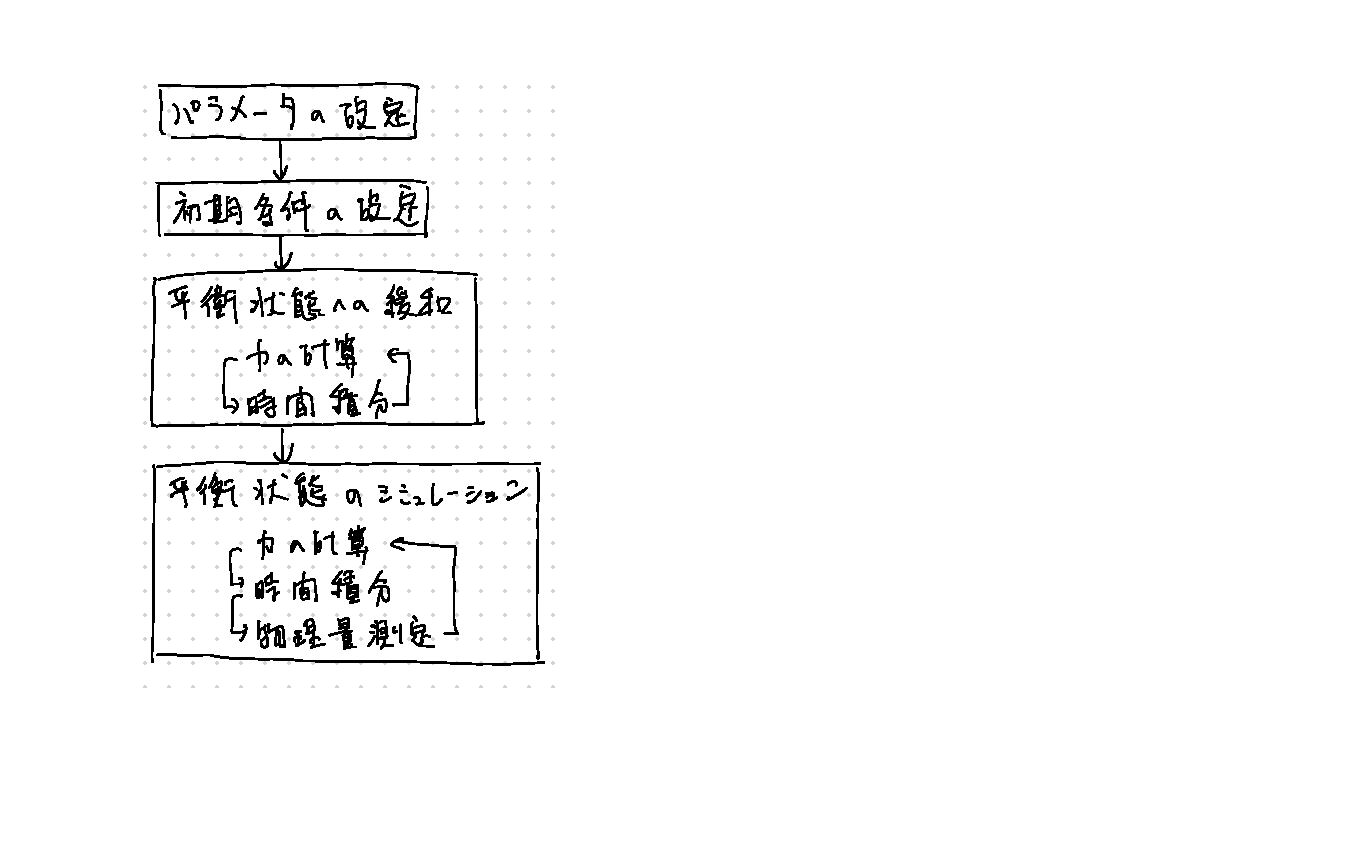
\includegraphics{image/md-flowchart.pdf}}
\end{center}
\end{frame}

% Adapted from molecular_dynamics-01.tex; ergodicity made explicit.
\begin{frame}{時間平均とミクロカノニカル平均}
\[
\langle A\rangle_E=
\frac{\int A(q,p)\,\delta(H(q,p)-E)\,dq\,dp}
{\int\delta(H(q,p)-E)\,dq\,dp}
\]
\[
\overline A_t=\frac{1}{t_{\max}}\int_0^{t_{\max}} A(q(t),p(t))\,dt
\]
\begin{itemize}
\item 孤立系の厳密な力学は、時間に依存しない $H$ を保存する
\item $\overline A_t\to\langle A\rangle_E$ には、対象とする不変集合上のエルゴード性が必要
\item 全運動量なども固定する場合、分布にその拘束を含める
\item エネルギー保存だけでは、平衡分布の十分な探索は保証されない
\end{itemize}
\end{frame}

\begin{frame}{孤立した調和振動子の例}
\[
H=\frac{p^2+q^2}{2}=E,\qquad
q(t)=\sqrt{2E}\cos(t+\phi)
\]
\[
P_E(q)=\frac{1}{\pi\sqrt{2E-q^2}}\quad (|q|<\sqrt{2E})
\]
\begin{itemize}
\item 一つのエネルギー軌道を何周しても、他のエネルギーには移らない
\item カノニカル分布の $q$ はガウス分布。固定エネルギーの分布とは異なる
\item 温度一定の標本を得るには、熱浴または確率的な更新が必要
\end{itemize}
\end{frame}

\section{シンプレクティック積分法}

% Adapted from symplectic-01.tex.
\begin{frame}{ハミルトン力学の構造}
\[
\frac{dH}{dt}=\sum_a\left(
\frac{\partial H}{\partial q_a}\dot q_a+
\frac{\partial H}{\partial p_a}\dot p_a\right)=0
\]
\[
\nabla\cdot\dot z=\sum_a\left(
\frac{\partial\dot q_a}{\partial q_a}+
\frac{\partial\dot p_a}{\partial p_a}\right)=0,
\qquad z=(q,p)
\]
\begin{itemize}
\item エネルギー保存と位相空間の体積保存（Liouvilleの定理）
\item 数値解法も、この構造をどこまで保持するか確認する
\item 通常の陽的Euler法や古典的4次Runge-Kutta法は、一般には保持しない
\end{itemize}
\end{frame}

\begin{frame}{陽的Euler法で調和振動子を解くと}
\[
\begin{pmatrix}q_{n+1}\\p_{n+1}\end{pmatrix}
=\begin{pmatrix}1&h\\-h&1\end{pmatrix}
\begin{pmatrix}q_n\\p_n\end{pmatrix}
\]
\[
\det D\Phi_h=1+h^2,\qquad H_{n+1}=(1+h^2)H_n
\]
\begin{itemize}
\item 位相空間の面積も、エネルギーも毎ステップ増える
\item $h$ を小さくすると有限時間の誤差は減るが、長時間では膨らみ続ける
\item 局所的な打切り誤差の次数だけでは、長時間の性質を判断できない
\end{itemize}
\end{frame}

% Adapted from symplectic-02.tex, symplectic-03.tex.
\begin{frame}{シンプレクティックEuler法}
\[
q_{n+1}=q_n+hp_n,\qquad p_{n+1}=p_n-hq_{n+1}
\]
\[
D\Phi_h=\begin{pmatrix}1&h\\-h&1-h^2\end{pmatrix},
\qquad \det D\Phi_h=1
\]
\[
\widetilde H=\frac{p^2+q^2+hpq}{2}
\]
\begin{itemize}
\item この調和振動子では $\widetilde H$ が厳密に保存される
\item $0<h<2$ なら $\widetilde H$ は正定値。$H$ の誤差は $O(h)$ の範囲で振動
\item 一次精度。時間反転対称な二次精度の方法も構成できる
\end{itemize}
\end{frame}

\begin{frame}{シンプレクティック性と体積保存}
\[
(D\Phi_h)^{\mathsf T}J(D\Phi_h)=J,
\qquad J=\begin{pmatrix}0&I\\-I&0\end{pmatrix}
\]
\begin{itemize}
\item シンプレクティック写像は、正準的な面積の構造を保存する
\item シンプレクティック性から位相空間の体積保存が従う
\item 複数自由度では、体積保存だけではシンプレクティックとは限らない
\item シンプレクティック性は、元の $H$ の厳密保存を意味しない
\end{itemize}
\end{frame}

% Adapted from symplectic-04.tex; explicit masses and corrected brackets.
\begin{frame}{リープフロッグ：kick--drift--kick}
\[
\begin{aligned}
p_{a,n+1/2}&=p_{a,n}+\frac{h}{2}F_a(q_n)\\
q_{a,n+1}&=q_{a,n}+h\frac{p_{a,n+1/2}}{m_a}\\
p_{a,n+1}&=p_{a,n+1/2}+\frac{h}{2}F_a(q_{n+1})
\end{aligned}
\]
\begin{itemize}
\item 運動量を半歩、位置を一歩、運動量を半歩進める
\item 各操作はシンプレクティック。逆順に $-h$ で戻すと元に戻る
\item 局所誤差 $O(h^3)$、固定した有限時間に対する大域誤差 $O(h^2)$
\end{itemize}
\end{frame}

% Adapted from symplectic-08.tex.
\begin{frame}{速度ベルレ法}
\[
\begin{aligned}
q_{a,n+1}&=q_{a,n}+h\frac{p_{a,n}}{m_a}
+\frac{h^2}{2m_a}F_a(q_n)\\
p_{a,n+1}&=p_{a,n}+\frac{h}{2}
\left[F_a(q_n)+F_a(q_{n+1})\right]
\end{aligned}
\]
\begin{itemize}
\item 半ステップの運動量を消去すると、リープフロッグと同じ更新になる
\item $q,p$ が同じ時刻で得られるので、エネルギー・温度の測定が容易
\item 前ステップの力を再利用すれば、1ステップにつき新しい力の計算は1回
\end{itemize}
\end{frame}

\begin{frame}{実装時に確認すること}
\begin{enumerate}
\item 初期状態の力 $F(q_0)$ を計算する
\item 全成分の運動量を半歩更新する
\item 全成分の位置を一歩更新し、必要なら周期境界処理をする
\item 新しい位置から全成分の力を再計算する
\item 運動量を残り半歩更新してから、物理量を測定する
\end{enumerate}
\begin{itemize}
\item 古い位置と新しい位置を混ぜて力を評価しない
\item $p$ と速度 $v=p/m$、力 $F$ と加速度 $F/m$ を区別する
\end{itemize}
\end{frame}

\begin{frame}{調和振動子のエネルギー誤差}
\begin{center}
\resizebox{0.85\textwidth}{!}{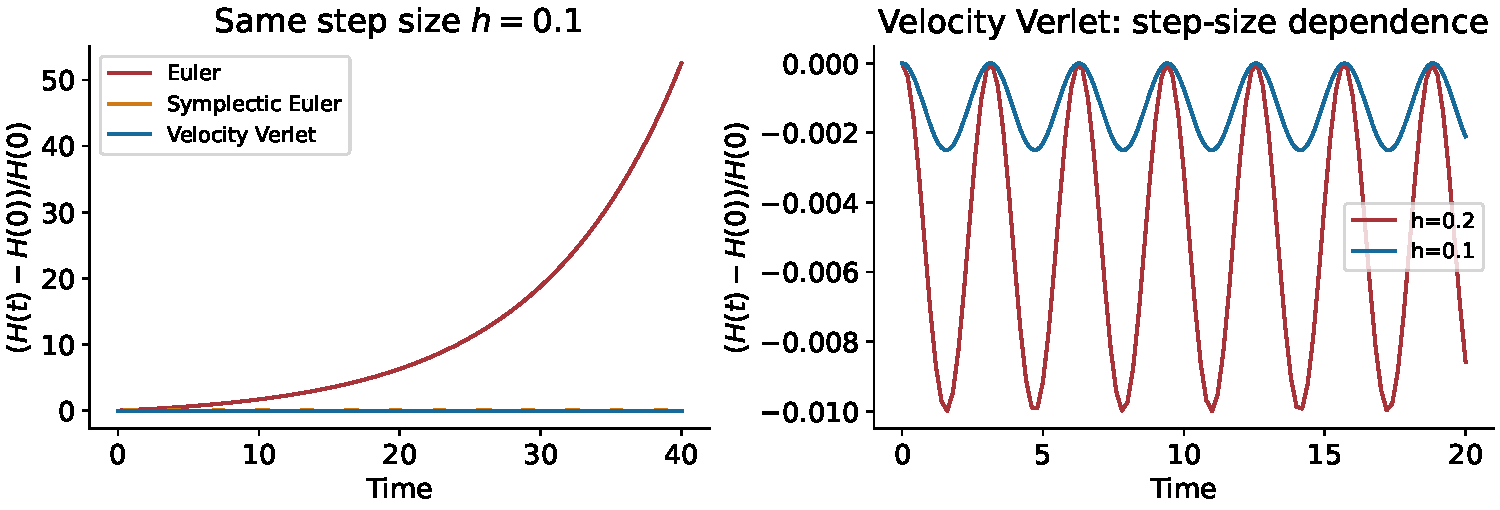
\includegraphics{image/md-2026-energy.pdf}}
\end{center}
\begin{itemize}
\item $m=k=1$, $q_0=1$, $p_0=0$。横軸は時間、縦軸は相対エネルギー誤差
\item ベルレ法では振動する誤差の幅が $h^2$ に比例する
\end{itemize}
\end{frame}

\begin{frame}{安定性と長時間計算}
\begin{itemize}
\item 調和振動子の速度ベルレ法は $0<h\omega<2$ で線形安定
\item 多粒子系では最も速い運動を解像する刻み幅が必要
\item 滑らかな $H$ と十分小さい固定刻み幅のもとで、修正ハミルトニアンを使って長時間のエネルギー誤差を説明できる
\item 衝突・特異点・不連続なカットオフ・大きすぎる刻み幅では破綻しうる
\item 状態に応じて単純に $h$ を変えると、通常はシンプレクティック性を失う
\end{itemize}
\end{frame}

\begin{frame}{数値積分の検証}
\begin{itemize}
\item 刻み幅 $h,h/2,h/4$ で同じ物理時刻まで計算する
\item 二次精度なら、漸近領域で有限時間の解の誤差はおよそ $1/4$ になる
\item エネルギー・全運動量のドリフトを調べる
\item $L$ ステップ進め、運動量を反転して $L$ ステップ進める
\end{itemize}
\[
R\Phi_h^L R\Phi_h^L(q,p)\simeq(q,p),\qquad R(q,p)=(q,-p)
\]
\begin{itemize}
\item 一致の限界は丸め誤差やカオスによる誤差増幅にも依存する
\end{itemize}
\end{frame}

\section{温度制御と統計的サンプリング}

% Adapted from virial-03.tex.
\begin{frame}{運動エネルギーから温度を測る}
\[
\langle K\rangle=\frac{f}{2}k_{\mathrm B}T,\qquad
T_{\mathrm{kin}}=\frac{2K}{f k_{\mathrm B}}
\]
\begin{itemize}
\item $f$ は独立な運動量の自由度数。拘束のない3次元系では $f=3N$
\item 全運動量を0に固定した場合は $f=3N-3$。他の拘束も差し引く
\item カノニカル分布では瞬間的な $T_{\mathrm{kin}}$ はゆらぐ
\end{itemize}
\[
\mathrm{Var}(K)=\frac{f}{2}(k_{\mathrm B}T)^2
\]
\begin{itemize}
\item 平均温度だけが一致しても、正しい分布を得たとはいえない
\end{itemize}
\end{frame}

% Adapted from molecular_dynamics-04.tex.
\begin{frame}{毎ステップの速度スケーリング}
\[
p_a\leftarrow\lambda p_a,\qquad
\lambda=\sqrt{\frac{f k_{\mathrm B}T}{2K}}
\]
\begin{itemize}
\item 更新直後は必ず $K=f k_{\mathrm B}T/2$ になる（$K>0$ の場合）
\item 運動エネルギーのゆらぎを消してしまう
\item この操作だけではカノニカル分布を生成しない
\item 初期緩和で用いても、測定に使う更新法と平衡化は別に検証する
\end{itemize}
\end{frame}

% Adapted from molecular_dynamics-05.tex; split the two methods.
\begin{frame}{Langevin熱浴}
\[
\dot q_a=\frac{p_a}{m_a},\qquad
\dot p_a=F_a(q)-\gamma_a p_a+R_a(t)
\]
\[
\langle R_a(t)\rangle=0,\qquad
\langle R_a(t)R_b(t')\rangle
=2m_a\gamma_a k_{\mathrm B}T\,\delta_{ab}\delta(t-t')
\]
\begin{itemize}
\item 摩擦による散逸と、雑音による揺動を対応させる
\item 連続時間の定常分布はカノニカル分布
\item 数値離散化には系統誤差がある。刻み幅依存性を確認する
\item 摩擦係数は緩和速度と動的相関を変える
\end{itemize}
\end{frame}

\begin{frame}{Andersen熱浴}
\begin{itemize}
\item Hamilton力学による時間発展と、熱浴とのランダムな衝突を組み合わせる
\item 刻み幅 $h$ の間に、粒子ごとに確率 $1-e^{-\nu h}$ で運動量を再抽選
\end{itemize}
\[
p_{i\alpha}\sim\mathcal N(0,m_i k_{\mathrm B}T)
\]
\begin{itemize}
\item $\nu h\ll1$ なら衝突確率は $\nu h$ と近似できる
\item 厳密なHamilton流と再抽選は、それぞれカノニカル分布を保つ
\item 数値積分の誤差は残る。衝突は全運動量を保存せず、動的性質も変える
\end{itemize}
\end{frame}

% Adapted from molecular_dynamics-08.tex and -14.tex.
\begin{frame}{Nosé--Hoover熱浴}
\[
\dot q_a=\frac{p_a}{m_a},\qquad
\dot p_a=F_a-\zeta p_a,\qquad
\dot\zeta=\frac{2K-f k_{\mathrm B}T}{Q}
\]
\begin{itemize}
\item $\zeta$：動的な摩擦係数。$Q>0$：熱浴の応答時間を決めるパラメータ
\item $K$ が大きいと $\zeta$ が増加し、運動量を抑える
\item 拡張位相空間の定常密度は
\end{itemize}
\[
\rho(q,p,\zeta)\propto
\exp\left[-\beta\left(H(q,p)+\frac{Q\zeta^2}{2}\right)\right]
\]
\end{frame}

\begin{frame}{定常分布とエルゴード性}
\begin{itemize}
\item 定常分布が正しくても、一つの軌道がその分布を探索するとは限らない
\item 単一のNosé--Hoover熱浴と調和振動子の組合せでは、非エルゴード的な挙動が起こりうる
\item 熱浴の連鎖や確率的熱浴を使う方法がある
\item 複数の初期条件から、分布・モーメント・自己相関を比較する
\item 平衡平均を求める目的と、物理的な輸送・緩和を調べる目的を区別する
\end{itemize}
\end{frame}

\begin{frame}{測定値の相関と誤差評価}
\[
C_A(t)=\frac{\langle A_i A_{i+t}\rangle-\langle A\rangle^2}{\sigma_A^2},
\qquad \tau_{\mathrm{int},A}=\sum_{t=1}^{\infty}C_A(t)
\]
\[
\mathrm{Var}(\overline A)\simeq
\frac{\sigma_A^2}{M}(1+2\tau_{\mathrm{int},A}),\qquad
M_{\mathrm{eff}}=\frac{M}{1+2\tau_{\mathrm{int},A}}
\]
\begin{itemize}
\item 講義1と同じ規約。$t$ は測定間隔を単位とするラグ
\item 平衡化後の定常な時系列で、十分長い測定を行う
\item ビン幅を変え、誤差の推定値が安定する範囲を探す
\item $q$ と $q^2$ では自己相関が異なる。負の相関にも注意する
\end{itemize}
\end{frame}

\section{Hamiltonian Monte Carlo}

% Adapted from hamiltonian_montecarlo-01.tex and -02.tex.
\begin{frame}{力学を使って候補を生成する}
\begin{itemize}
\item ランダムウォーク型Metropolis法は、細長い分布の探索が遅くなりやすい
\item 仮想的な運動量を導入し、勾配を使って連続的に移動する
\item 数値積分で生成した候補を、Metropolis法で採択・棄却する
\item 標準的なHMCは、微分可能な対数密度をもつ連続変数が対象
\item 拘束のある変数には、座標変換や拘束を保つ積分法が必要
\end{itemize}
\end{frame}

\begin{frame}{拡張分布と仮想ハミルトニアン}
\[
\pi(q)\propto e^{-S(q)},\qquad
\mathcal H(q,p)=S(q)+\frac12 p^{\mathsf T}\mathsf M^{-1}p
\]
\[
\Pi(q,p)\propto e^{-\mathcal H(q,p)},\qquad
p\sim\mathcal N(0,\mathsf M)
\]
\begin{itemize}
\item $S(q)=-\log\pi(q)+\mathrm{const}$。物理の分布なら $S=\beta U$
\item $\mathcal H$ は無次元。採択確率に $\beta$ をもう一度掛けない
\item $\mathsf M$ は一定の正定値行列。$p$ を積分すると元の $\pi(q)$ を得る
\item 仮想時間の運動方程式：$\dot q=\mathsf M^{-1}p$, $\dot p=-\nabla S(q)$
\end{itemize}
\end{frame}

\begin{frame}{HMCの1ステップ}
\begin{enumerate}
\item 現在の $q$ を保存し、$p\sim\mathcal N(0,\mathsf M)$ を新たに生成する
\item $\mathcal H_0=\mathcal H(q,p)$ を計算する
\item 刻み幅 $h$ のリープフロッグを $L$ 回適用する
\item 最終運動量を反転し、候補 $(q^*,p^*)$ とする
\item 次の確率で候補を採択する
\end{enumerate}
\[
\alpha=\min\left(1,e^{-\Delta\mathcal H}\right),\qquad
\Delta\mathcal H=\mathcal H(q^*,p^*)-\mathcal H_0
\]
\begin{itemize}
\item 棄却時は元の $q$ に戻す。採択・棄却のどちらでも $q$ を測定する
\end{itemize}
\end{frame}

\begin{frame}{可逆性・体積保存と採択確率}
\[
R(q,p)=(q,-p),\quad \Psi=R\Phi_h^L,\quad
\Psi^2=I,\quad |\det D\Psi|=1
\]
\begin{itemize}
\item 運動量反転を含む提案は対合：同じ操作で元に戻る
\item 体積保存により、変数変換のJacobian因子は1
\item $z' =\Psi z$ の組に対して、確率流は
\end{itemize}
\[
e^{-\mathcal H(z)}\min(1,e^{-\mathcal H(z')+\mathcal H(z)})
=\min(e^{-\mathcal H(z)},e^{-\mathcal H(z')})
\]
\begin{itemize}
\item 右辺は $z,z'$ の交換で不変。体積保存だけではこの議論は完成しない
\end{itemize}
\end{frame}

\begin{frame}{Metropolis補正の役割}
\begin{itemize}
\item 厳密なHamilton流なら $\Delta\mathcal H=0$、候補を常に採択できる
\item 数値積分では $\Delta\mathcal H\ne0$。採択・棄却が定常分布の偏りを補正する
\item 可逆性と体積保存、正しいエネルギー差評価が前提
\item 補正しても、有限標本の統計誤差や平衡化不足は残る
\item 数値的には $\log u<\min(0,-\Delta\mathcal H)$ を判定する
\end{itemize}
\[
u\sim\mathrm{Uniform}(0,1)
\]
\end{frame}

\begin{frame}{調和振動子で標本分布を確かめる}
\begin{center}
\resizebox{0.82\textwidth}{!}{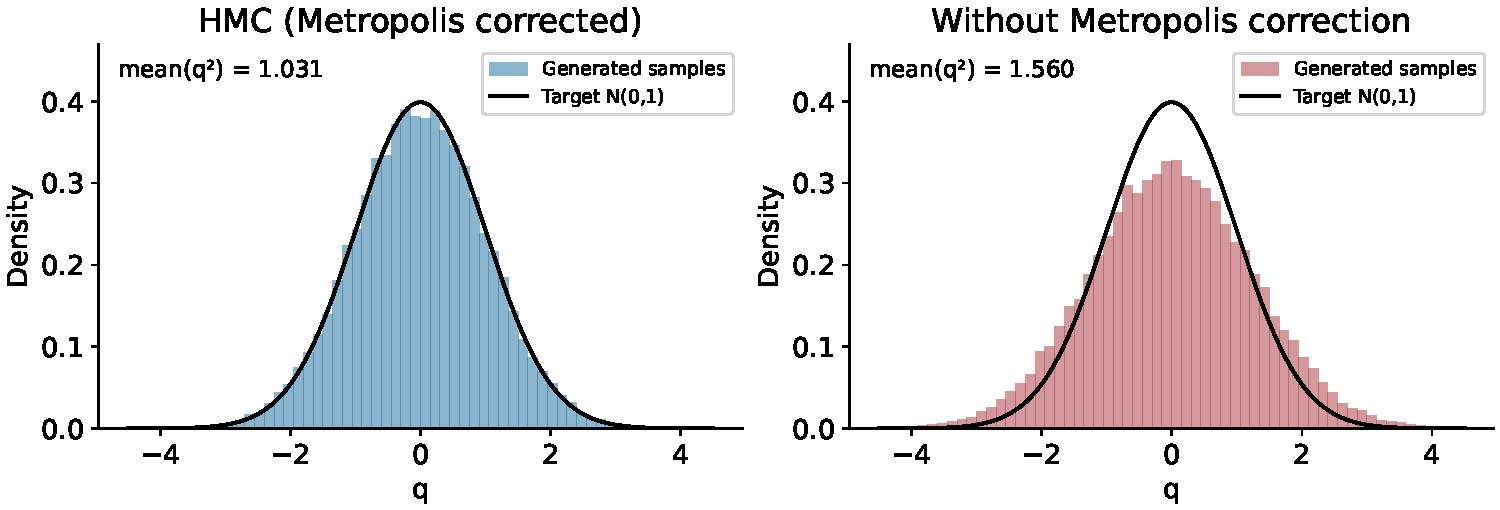
\includegraphics{image/md-2026-sampling.pdf}}
\end{center}
\begin{itemize}
\item $S=q^2/2$, $\mathsf M=1$。目標は $\langle q\rangle=0$, $\langle q^2\rangle=1$
\item 同じ $h,L$ でも採択・棄却を省くと分布がずれる
\end{itemize}
\end{frame}

\begin{frame}{刻み幅・軌道長・質量行列}
\begin{itemize}
\item $h$：積分誤差と採択率を変える。小さいほど計算回数が増える
\item $L$ と軌道長 $\tau=Lh$：移動距離と計算コストを変える
\item 長すぎる軌道は元に戻ることがあり、計算が無駄になる
\item 状態に依存しない分布から $L$ を選ぶと、周期との共鳴を避けやすい
\item $\mathsf M$：方向ごとの時間尺度を調整する
\end{itemize}
\[
S(q)=\frac12q^{\mathsf T}Aq\quad\Longrightarrow\quad
\ddot q=-\mathsf M^{-1}Aq
\]
\end{frame}

\begin{frame}{採択率だけでは効率を判断できない}
\begin{itemize}
\item ほとんど動かない提案でも採択率は高くなる
\item $q^2$ やエネルギーなど、目的の物理量の自己相関を調べる
\item 同じ計算時間、または同じ勾配評価回数で比較する
\item 多峰分布の山と山の間の移動は、HMCでも難しい場合がある
\item 初期条件・乱数seed・$h,L$ を変えて結果を照合する
\end{itemize}
\[
\text{効率の指標：}\quad
\frac{M_{\mathrm{eff}}}{\text{計算時間}}
\]
\end{frame}

\begin{frame}{分子動力学とHMCの役割}
\begin{itemize}
\item 孤立系MD：保存則のある時間発展。条件が整えばミクロカノニカル平均
\item 熱浴つきMD：カノニカル分布を目指す。熱浴と離散化を検証する
\item HMC：仮想力学で候補を作り、Metropolis補正で目標分布を保つ
\item HMCのステップ数は物理的な実時間ではない
\item どの場合も、探索不足と統計誤差を別に評価する
\end{itemize}
\end{frame}

\section{まとめと実習への接続}

\begin{frame}{実習2に向けた確認課題}
\begin{enumerate}
\item 調和振動子をEuler法・速度ベルレ法で積分し、$H(t)$ を比較する
\item $h$ を半分にして、誤差の減少と時間反転を確認する
\item HMCを実装し、$q$ のヒストグラムと $\langle q^2\rangle$ を確認する
\item 棄却された状態も含む時系列をビニングし、誤差を見積もる
\item 発展：局所Metropolis法と、勾配評価回数・時間あたりの効率を比較する
\end{enumerate}
\begin{itemize}
\item 実習2は10月30日（金）。提出条件は別途配布する実習資料を参照
\end{itemize}
\end{frame}

\begin{frame}{本日の要点}
\begin{itemize}
\item 保存量と刻み幅依存性から、数値積分の妥当性を確認する
\item シンプレクティック性・可逆性は、長時間積分とHMCを支える
\item 温度制御では、平均値・ゆらぎ・エルゴード性を区別する
\item HMCは、運動量再抽選・力学による提案・Metropolis補正を組み合わせる
\item 正しい定常分布と、有限時間での効率のよい探索は別の条件
\end{itemize}
\end{frame}

\section{補足}

% Adapted from virial-01.tex and virial-03.tex.
\begin{frame}{補足：ビリアル定理と圧力}
\[
G=\sum_i\mathbf p_i\cdot\mathbf r_i,\qquad
\dot G=2K+\sum_i\mathbf r_i\cdot\mathbf F_i
\]
\begin{itemize}
\item 束縛された系で $[G(t)-G(0)]/t\to0$ なら、$\langle\dot G\rangle=0$
\item 等方圧力の3次元粒子系では（対相互作用）
\end{itemize}
\[
P=\frac{1}{3V}\left(2\langle K\rangle+
\left\langle\sum_{i<j}\mathbf r_{ij}\cdot\mathbf F_{ij}\right\rangle\right)
\]
\begin{itemize}
\item 周期境界では、力の計算と整合する相対座標 $\mathbf r_{ij}$ を用いる
\item 周期的に折り返した絶対座標を、そのまま $G$ に代入しない
\end{itemize}
\end{frame}

% Adapted from longrange-01.tex; retain the original evidence figure.
\begin{frame}{補足：長距離力とエバルト分割}
\[
\frac1r=\frac{\mathrm{erfc}(\alpha r)}r+
\frac{\mathrm{erf}(\alpha r)}r
\]
\begin{center}
\resizebox{!}{0.40\textheight}{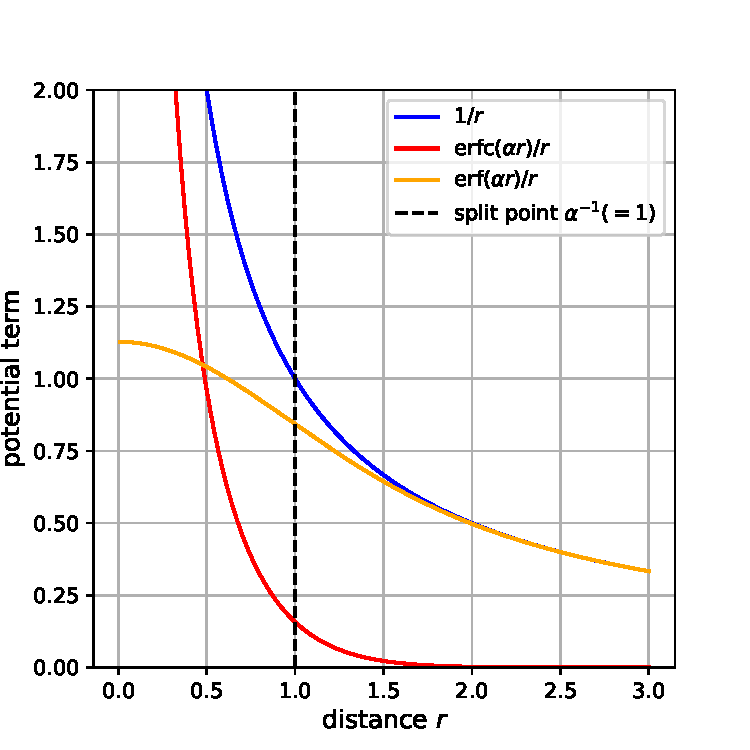
\includegraphics{image/ewald.pdf}}
\end{center}
\begin{itemize}
\item 短距離側を実空間、滑らかな長距離側を逆格子空間で計算する
\item 周期クーロン系では、自己項・中性条件・境界条件も指定する
\end{itemize}
\end{frame}

% Adapted from longrange-03.tex and -04.tex.
\begin{frame}{補足：ツリー法}
\begin{center}
\resizebox{!}{0.40\textheight}{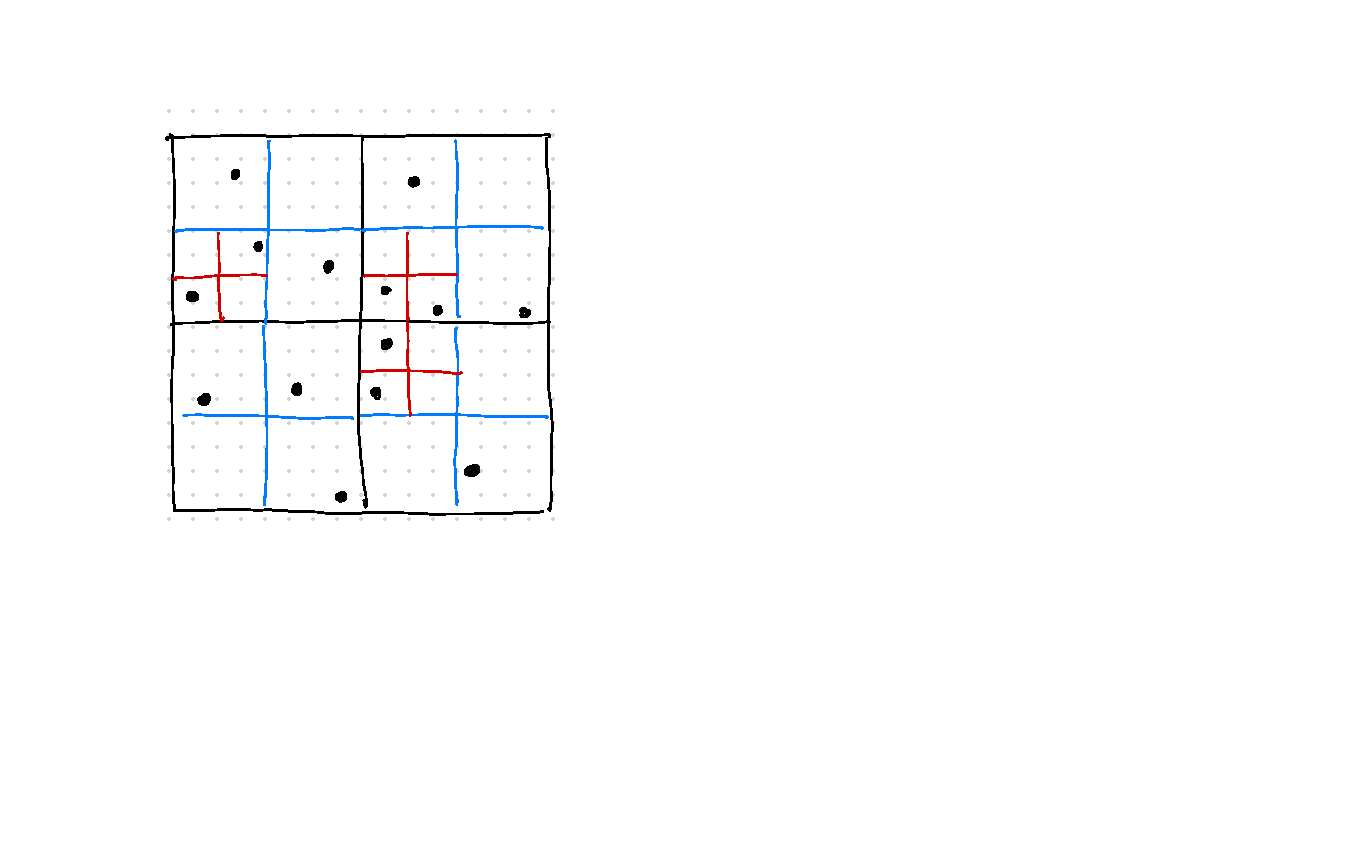
\includegraphics{image/tree-1.pdf}}
\resizebox{!}{0.40\textheight}{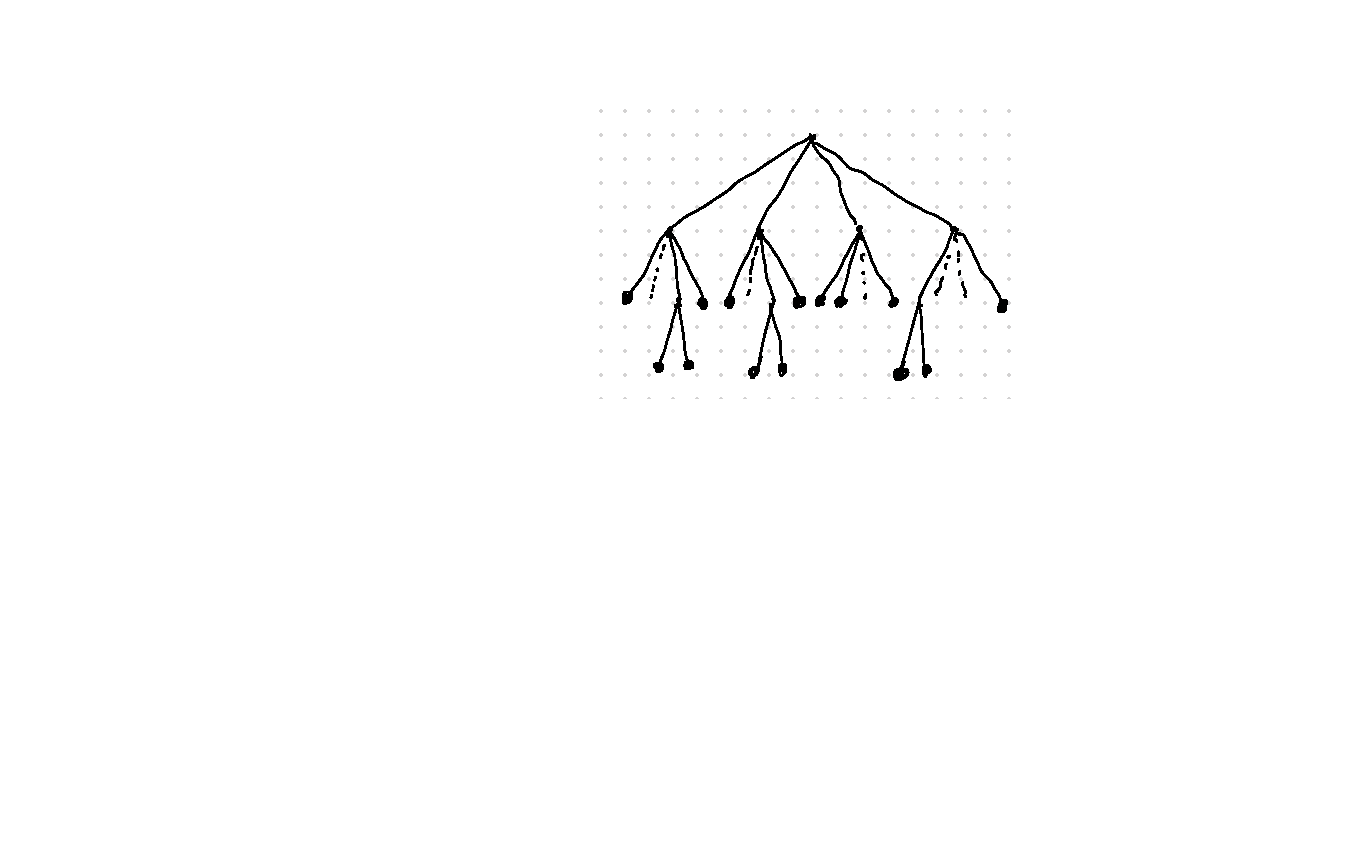
\includegraphics{image/tree-2.pdf}}
\end{center}
\begin{itemize}
\item 空間を再帰的に分割し、遠方の粒子群をまとめて近似する
\item 見込み角の閾値を小さくすると、精度と計算量がともに増す
\item 典型的な計算量は $O(N\log N)$。分布や精度条件に依存する
\end{itemize}
\end{frame}

% Adapted from symplectic-09.tex through -12.tex; use maps, not ambiguous operator order.
\begin{frame}{補足：分割法と四次の構成}
\[
A_h(q,p)=(q+h\nabla K(p),p),\qquad
B_h(q,p)=(q,p-h\nabla U(q))
\]
\[
S_2(h)=B_{h/2}\circ A_h\circ B_{h/2}
\]
\[
S_4(h)=S_2(w_1h)\circ S_2(w_0h)\circ S_2(w_1h)
\]
\[
w_1=\frac{1}{2-2^{1/3}},\qquad
w_0=-\frac{2^{1/3}}{2-2^{1/3}}
\]
\begin{itemize}
\item $2w_1+w_0=1$, $2w_1^3+w_0^3=0$。負の部分ステップを含む
\item 高次化では、力の評価回数と誤差減少の両方を比較する
\end{itemize}
\end{frame}

\begin{frame}{補足：Nosé--Hooverの定常密度}
\begin{itemize}
\item 拡張変数を $x=(q,p,\zeta)$ とすると、流れの発散は $-f\zeta$
\item 本編の密度 $\rho$ について、軌道に沿う変化を計算する
\end{itemize}
\[
\frac{d}{dt}\left(H+\frac{Q\zeta^2}{2}\right)
=-2K\zeta+\zeta(2K-f k_{\mathrm B}T)
=-f k_{\mathrm B}T\zeta
\]
\[
\frac{d\log\rho}{dt}=f\zeta=-\nabla\cdot\dot x
\]
\begin{itemize}
\item 定常Liouville方程式 $\nabla\cdot(\rho\dot x)=0$ を満たす
\item これは定常密度の確認であり、エルゴード性の証明ではない
\end{itemize}
\end{frame}

\begin{frame}{参考文献}
\begin{itemize}
\item R. M. Neal, MCMC using Hamiltonian dynamics (2011),
\url{https://arxiv.org/abs/1206.1901}
\item W. G. Hoover, Canonical dynamics: Equilibrium phase-space distributions,
Phys. Rev. A 31, 1695 (1985),
\url{https://doi.org/10.1103/PhysRevA.31.1695}
\item H. Yoshida, Construction of higher order symplectic integrators,
Phys. Lett. A 150, 262 (1990),
\url{https://doi.org/10.1016/0375-9601(90)90092-3}
\end{itemize}
\end{frame}

\end{document}
